\documentclass{article}[12pt]

% General packages
\usepackage[english]{babel}
\pagenumbering{arabic}
\usepackage{color}
\usepackage{lettrine}
\usepackage{setspace}
\usepackage{yfonts}
\usepackage{type1cm}


% Graphics packages
\usepackage{graphicx}
\usepackage{rotating}


% Math packages
\usepackage{array}
\usepackage{amsmath}
\usepackage{amsfonts}
\usepackage{amssymb}
\usepackage{geometry}
\usepackage{xparse}
\usepackage{physics}

% Links packages
\usepackage{hyperref}
\usepackage{url}
\usepackage{xcolor}
\hypersetup{
    colorlinks,
    linkcolor={blue!80!black},
    citecolor={blue!80!black},
    urlcolor={blue!80!black}
}


% Tables packages
\usepackage{adjustbox}
\usepackage{multirow}
\usepackage{hhline}
\usepackage{float}
\usepackage[bottom]{footmisc}
\usepackage{booktabs,caption}
\usepackage[flushleft]{threeparttable}
\usepackage[labelfont=sc]{caption}
\captionsetup[table]{skip=0pt}


% citations
\usepackage[round]{natbib}   % omit 'round' option if you prefer square brackets
%\bibliographystyle{plainnat}
%\bibliographystyle{abbrv}
%\bibliographystyle{acm}
%\bibliographystyle{alpha}
\bibliographystyle{apalike}
%\bibliographystyle{ieeetr}
%\bibliographystyle{plain}
%\bibliographystyle{siam}
%\bibliographystyle{unsrt}

% figures
\usepackage{subcaption}


\begin{document}

\title{Problem Set 3}
\author{Angela Shoulders}
\date{September 21, 2021}

\maketitle

Figure \ref{fig:tax2} uses data from the Tax Introduction Database.
This database includes information on when different types of taxes
were introduced in different countries.  This particular sample is
from 1850 to 2000 and includes 18 countries: Argentina, Australia,
Brazil, Canada, Chile, Columbia,Denmark, Finland, Ireland, Japan,
Mexico, Netherlands, New Zealand, Norway, Sweden, Switzerland,
the United Kingdom, and the United States.  It shows that countries
tend to implement an income tax first, and most countries had instituted
an income tax by the 1940s.  In the 1960s and 70s, countries tend
to start implementing a value added tax (VAT), though not all countries
have started collecting this tax yet.

Figure \ref{fig:IL} uses data from the Behavioral Risk Factor Surveillance
System (BRFSS).  This data includes a variety of physical and mental
health related variables, including the number of days of poor mental
health respondents have experienced in the last month.  I previously
have combined and collapsed this data to find the percentage of the
population by state, month, and year who experienced 0 poor mental
health days, 0-14 poor mental health days, and 14+ poor mental health
days.  This figure looks at the proportion of these three groups over
time in Illinois.  Clearly, something is amiss in the early 2000s,
which you can see by the massive dip in all groups.  My coauthor and
myself are working to discover the reason for this issue.  Generally,
however, we can see that the proportion of people with poor mental health
is trending up, while the proportion of people with good mental health
is trending down slightly.

Figure \ref{fig:mental} also uses BRFSS data, but looks at the percentage
of people experiencing 14+ poor mental health days in January of 2019
across all states.  We see that generally Northeastern and Western states
have the smallest mentally ill populations, while Southern and Midwestern
states have the largest mentally ill populations.

\begin{figure}
    \centering
    \caption{\textsc{Adoption of Different Tax Types}}
    \label{fig:tax2}
    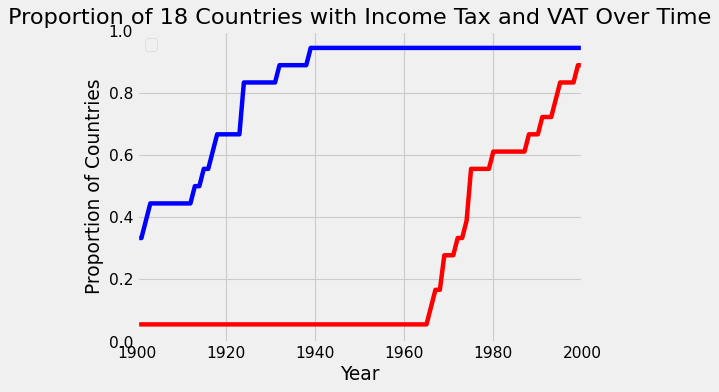
\includegraphics[scale=0.6]{tax.png}
    \hspace{0.5cm}
\end{figure}

\begin{figure}
    \centering
    \caption{\textsc{Evolution of Mental Health in Illinois}}
    \label{fig:IL}
    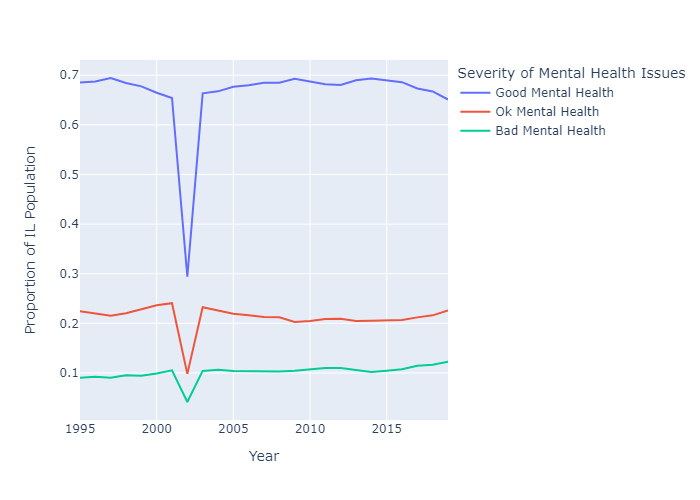
\includegraphics[scale=0.6]{fig2.png}
    \hspace{0.5cm}
\end{figure}

\begin{figure}
    \centering
    \caption{\textsc{Proportion of Population with 14+ Bad Mental Health Days in January 2019}}
    \label{fig:mental}
    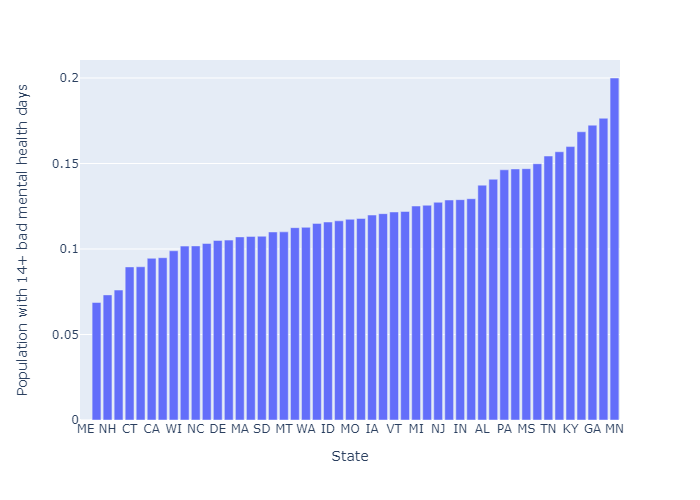
\includegraphics[scale=0.6]{fig3.png}
    \hspace{0.5cm}
\end{figure}


\end{document}